%% The first command in your LaTeX source must be the \documentclass command.
%%%% Small single column format, used for CIE, CSUR, DTRAP, JACM, JDIQ, JEA, JERIC, JETC, PACMCGIT, TAAS, TACCESS, TACO, TALG, TALLIP (formerly TALIP), TCPS, TDSCI, TEAC, TECS, TELO, THRI, TIIS, TIOT, TISSEC, TIST, TKDD, TMIS, TOCE, TOCHI, TOCL, TOCS, TOCT, TODAES, TODS, TOIS, TOIT, TOMACS, TOMM (formerly TOMCCAP), TOMPECS, TOMS, TOPC, TOPLAS, TOPS, TOS, TOSEM, TOSN, TQC, TRETS, TSAS, TSC, TSLP, TWEB.
% \documentclass[acmsmall]{acmart}

%%%% Large single column format, used for IMWUT, JOCCH, PACMPL, POMACS, TAP, PACMHCI
% \documentclass[acmlarge,screen]{acmart}

%%%% Large double column format, used for TOG
% \documentclass[acmtog, authorversion]{acmart}

%%%% Generic manuscript mode, required for submission
%%%% and peer review
\documentclass[manuscript, anonymous, review]{acmart}
\usepackage{todonotes}
\usepackage{xcolor}
% \usepackage{graphicx}
% \graphicspath{ {./images/} }
\usepackage{caption}
\usepackage{subcaption}
%% Fonts used in the template cannot be substituted; margin 
%% adjustments are not allowed.
%%
%% \BibTeX command to typeset BibTeX logo in the docs
\AtBeginDocument{%
  \providecommand\BibTeX{{%
    \normalfont B\kern-0.5em{\scshape i\kern-0.25em b}\kern-0.8em\TeX}}}

%% Rights management information.  This information is sent to you
%% when you complete the rights form.  These commands have SAMPLE
%% values in them; it is your responsibility as an author to replace
%% the commands and values with those provided to you when you
%% complete the rights form.
\setcopyright{acmcopyright}
\copyrightyear{2018}
\acmYear{2018}
\acmDOI{XXXXXXX.XXXXXXX}

%% These commands are for a PROCEEDINGS abstract or paper.
\acmConference[Conference acronym 'XX]{Make sure to enter the correct conference title from your rights confirmation emai}{June 03--05,
  2018}{Woodstock, NY}


\acmBooktitle{Woodstock '18: ACM Symposium on Neural Gaze Detection, June 03--05, 2018, Woodstock, NY} 
\acmPrice{15.00}
\acmISBN{978-1-4503-XXXX-X/18/06}


%%
%% Submission ID.
%% Use this when submitting an article to a sponsored event. You'll
%% receive a unique submission ID from the organizers
%% of the event, and this ID should be used as the parameter to this command.
%%\acmSubmissionID{123-A56-BU3}

%%
%% end of the preamble, start of the body of the document source.
\begin{document}

%%
%% The "title" command has an optional parameter,
%% allowing the author to define a "short title" to be used in page headers.
\title{Material Experience Design for Smart Built Environments}

%%
%% The "author" command and its associated commands are used to define
%% the authors and their affiliations.
%% Of note is the shared affiliation of the first two authors, and the
%% "authornote" and "authornotemark" commands
%% used to denote shared contribution to the research.
\author{Shruti Rao}
\email{s.rao@uva.nl}
\orcid{1234-5678-9012}
\affiliation{
  \institution{University of Amsterdam}
  \city{Amsterdam}
  \country{The Netherlands}
}



%%
%% By default, the full list of authors will be used in the page
%% headers. Often, this list is too long, and will overlap
%% other information printed in the page headers. This command allows
%% the author to define a more concise list
%% of authors' names for this purpose.
\renewcommand{\shortauthors}{Rao et al.}

%%
%% The abstract is a short summary of the work to be presented in the
%% article.
\begin{abstract}
%   Abstracts should be about 150 words.
Given that people spend a significant amount of time within ``smart built spaces", designing spaces considering the impact that it may have on occupants’ comfort and emotions is a challenge for Human-Building Interaction (HBI). In this position paper, we offer the view of designing smart learning environments through the lens of material experiences design, whereby materials (both tangible and intangible) may impact occupants experiences of comfort and emotions. To that end, we describe our case study and how our expected findings may aid in identification of novel, subjective human experiences (sensory, affective, interpretive and performative) with materials in hybrid spaces. These cues may serve as a preliminary step towards designing comfort-enabling materials  and experiences in a smart, hybrid learning environment. 
\end{abstract}

%%
%% The code below is generated by the tool at http://dl.acm.org/ccs.cfm.
%% Please copy and paste the code instead of the example below.
%%

\begin{CCSXML}
<ccs2012>
   <concept>
       <concept_id>10003120</concept_id>
       <concept_desc>Human-centered computing</concept_desc>
       <concept_significance>500</concept_significance>
       </concept>
   <concept>
       <concept_id>10003120.10003123</concept_id>
       <concept_desc>Human-centered computing~Interaction design</concept_desc>
       <concept_significance>500</concept_significance>
       </concept>
 </ccs2012>
\end{CCSXML}

\ccsdesc[500]{Human-centered computing}
\ccsdesc[500]{Human-centered computing~Interaction design}

%%
%% Keywords. The author(s) should pick words that accurately describe
%% the work being presented. Separate the keywords with commas.
\keywords{affective computing, comfort, smart built environments, material experiences, body perception}

%% A "teaser" image appears between the author and affiliation
%% information and the body of the document, and typically spans the
%% page.
% \begin{teaserfigure}
%   \includegraphics[width=\textwidth]{sampleteaser}
%   \caption{Seattle Mariners at Spring Training, 2010.}
%   \Description{Enjoying the baseball game from the third-base
%   seats. Ichiro Suzuki preparing to bat.}
%   \label{fig:teaser}
% \end{teaserfigure}

 
%%
%% This command processes the author and affiliation and title
%% information and builds the first part of the formatted document.
\maketitle

\section{Introduction}
% Architecture + smart buildings
The evolution of information and communication technologies (ICT), building energy management systems (BEMS), and sustainability sciences have transformed buildings into thoughtful, sustainable, digital, interactive objects \cite{nembrini2017human}. These ``smart built environments" have presented an opportunity for human-computer interaction (HCI) research to bridge the gap between intelligent designs, sustainability goals and human needs in such built environments.  

% Materials in Architecture and buildings
Throughout the discourse of architecture, materials have been considered the language and expression of buildings. The role of materials and materiality in particular have been questioned during periods of new material development and changing technological capabilities. Advancements in technology has dramatically enhanced material capabilities that can now be used to support, emit, store, simulate, infer, inform and even create. Much of the smart materials abilities lie in their ability to change property over time

% Role of humans (body) in architecture and materials
The human body lies at the intersection of architecture and materials where both coincide to interact with the human. The changing nature of materials and therefore the spaces that encompass them may create unfamiliar and novel human-human and human-machine interactions and warrant further exploration. % impact humans' comfort in the broadest sense (phycially and emotionally).   

% position
% In this position paper, we consider comfort of occupants in its broadest sense - a physical and emotional manifestation. 
In this position paper, we consider an HCI-based approach on materials and materiality. We posit that architecture in the digital age should be examined through the lens of the material expressions framework. We believe that the material experience framework may provide a more holistic, user-centric, and technology imbibed methodology to examine the impact of architecture on its occupants. 

% paper outline]
\todo{outline needs to be updated}
We next provide a background on the material expressions framework.

The remainder of this paper then describes our case study as a first step towards understanding the role of materiality of artifacts in architecture, and the contributions our findings can make towards the comfort-enabling material experiences in hybrid learning spaces.


\section{Background}
% Comfort in Architecture
The concept of comfort is central to occupants within built environments. Comfort is understood as occupants' physiological and affective (emotional) responses to the built environment \cite{alavi2017comfort}. HBI especially examines the relationship between occupant comfort and four physical characteristics of the indoor environment - temperature, air, light, and sound \cite{hawkes2007environmental, bluyssen2009indoor}. 

% Examples of existing work
Much of the work in comfort studies focus on designing ``optimally informative" systems such as temperature calendars, air quality forecasts, noise level indicators, and wearables that appropriately inform occupants of their environment and also allow them to engage with comfort parameters to certain degrees  \cite{costanza2016bit, milenkovic2013improving, kim2020designing}. Other works focus on a ``gamified" approach to engage users with their environment and activities in a socially inclusive manner \cite{mathur2015tiny, kwallek1997impact, zhong2022augmenting}. 

% Our perspective
Therefore, to our knowledge comfort studies tend to focus on designing novel interfaces and digital systems for occupants. Instead, in this position paper we wish to reconsider designing for occupants' affective and physical comfort through the lens of materials and material experiences of tangible and intangible artifacts in a smart hybrid learning environment. 


\section{Material Experiences Design For Architecture in the Digital Age}

% Why should we design keeping in mind materiality
A significant consequence of smart buildings is that occupants find themselves physically immersed within a digital object, and therefore experience interactions in a novel, multi-sensory manner \cite{nembrini2017human}. 
% Moreover, providing for subjective comfort to occupants within a hybrid space that is used by different people with varying usage goals remains a relevant question. 

We believe that the materials experience framework can be used as a novel means to understand the relationship between materials and occupants at different experiential levels (sensorial, affective, interpretive and performative) within hybrid spaces \cite{giaccardi2015foundations}. Different tangible and intangible materials in hybrid spaces can be utilised to shape the ways in which occupants experience emotional and physical comfort, and consequently learning attitudes. Moreover, material
experiences can play a more ubiquitous role in fostering occupants' interactions with non-digital elements of the building through digital means - a key concern in HBI \cite{nembrini2017human}. 

\subsection{A Digital Building of the Present}

% \begin{figure}[h]
%   \centering
%   \begin{subfigure}
%   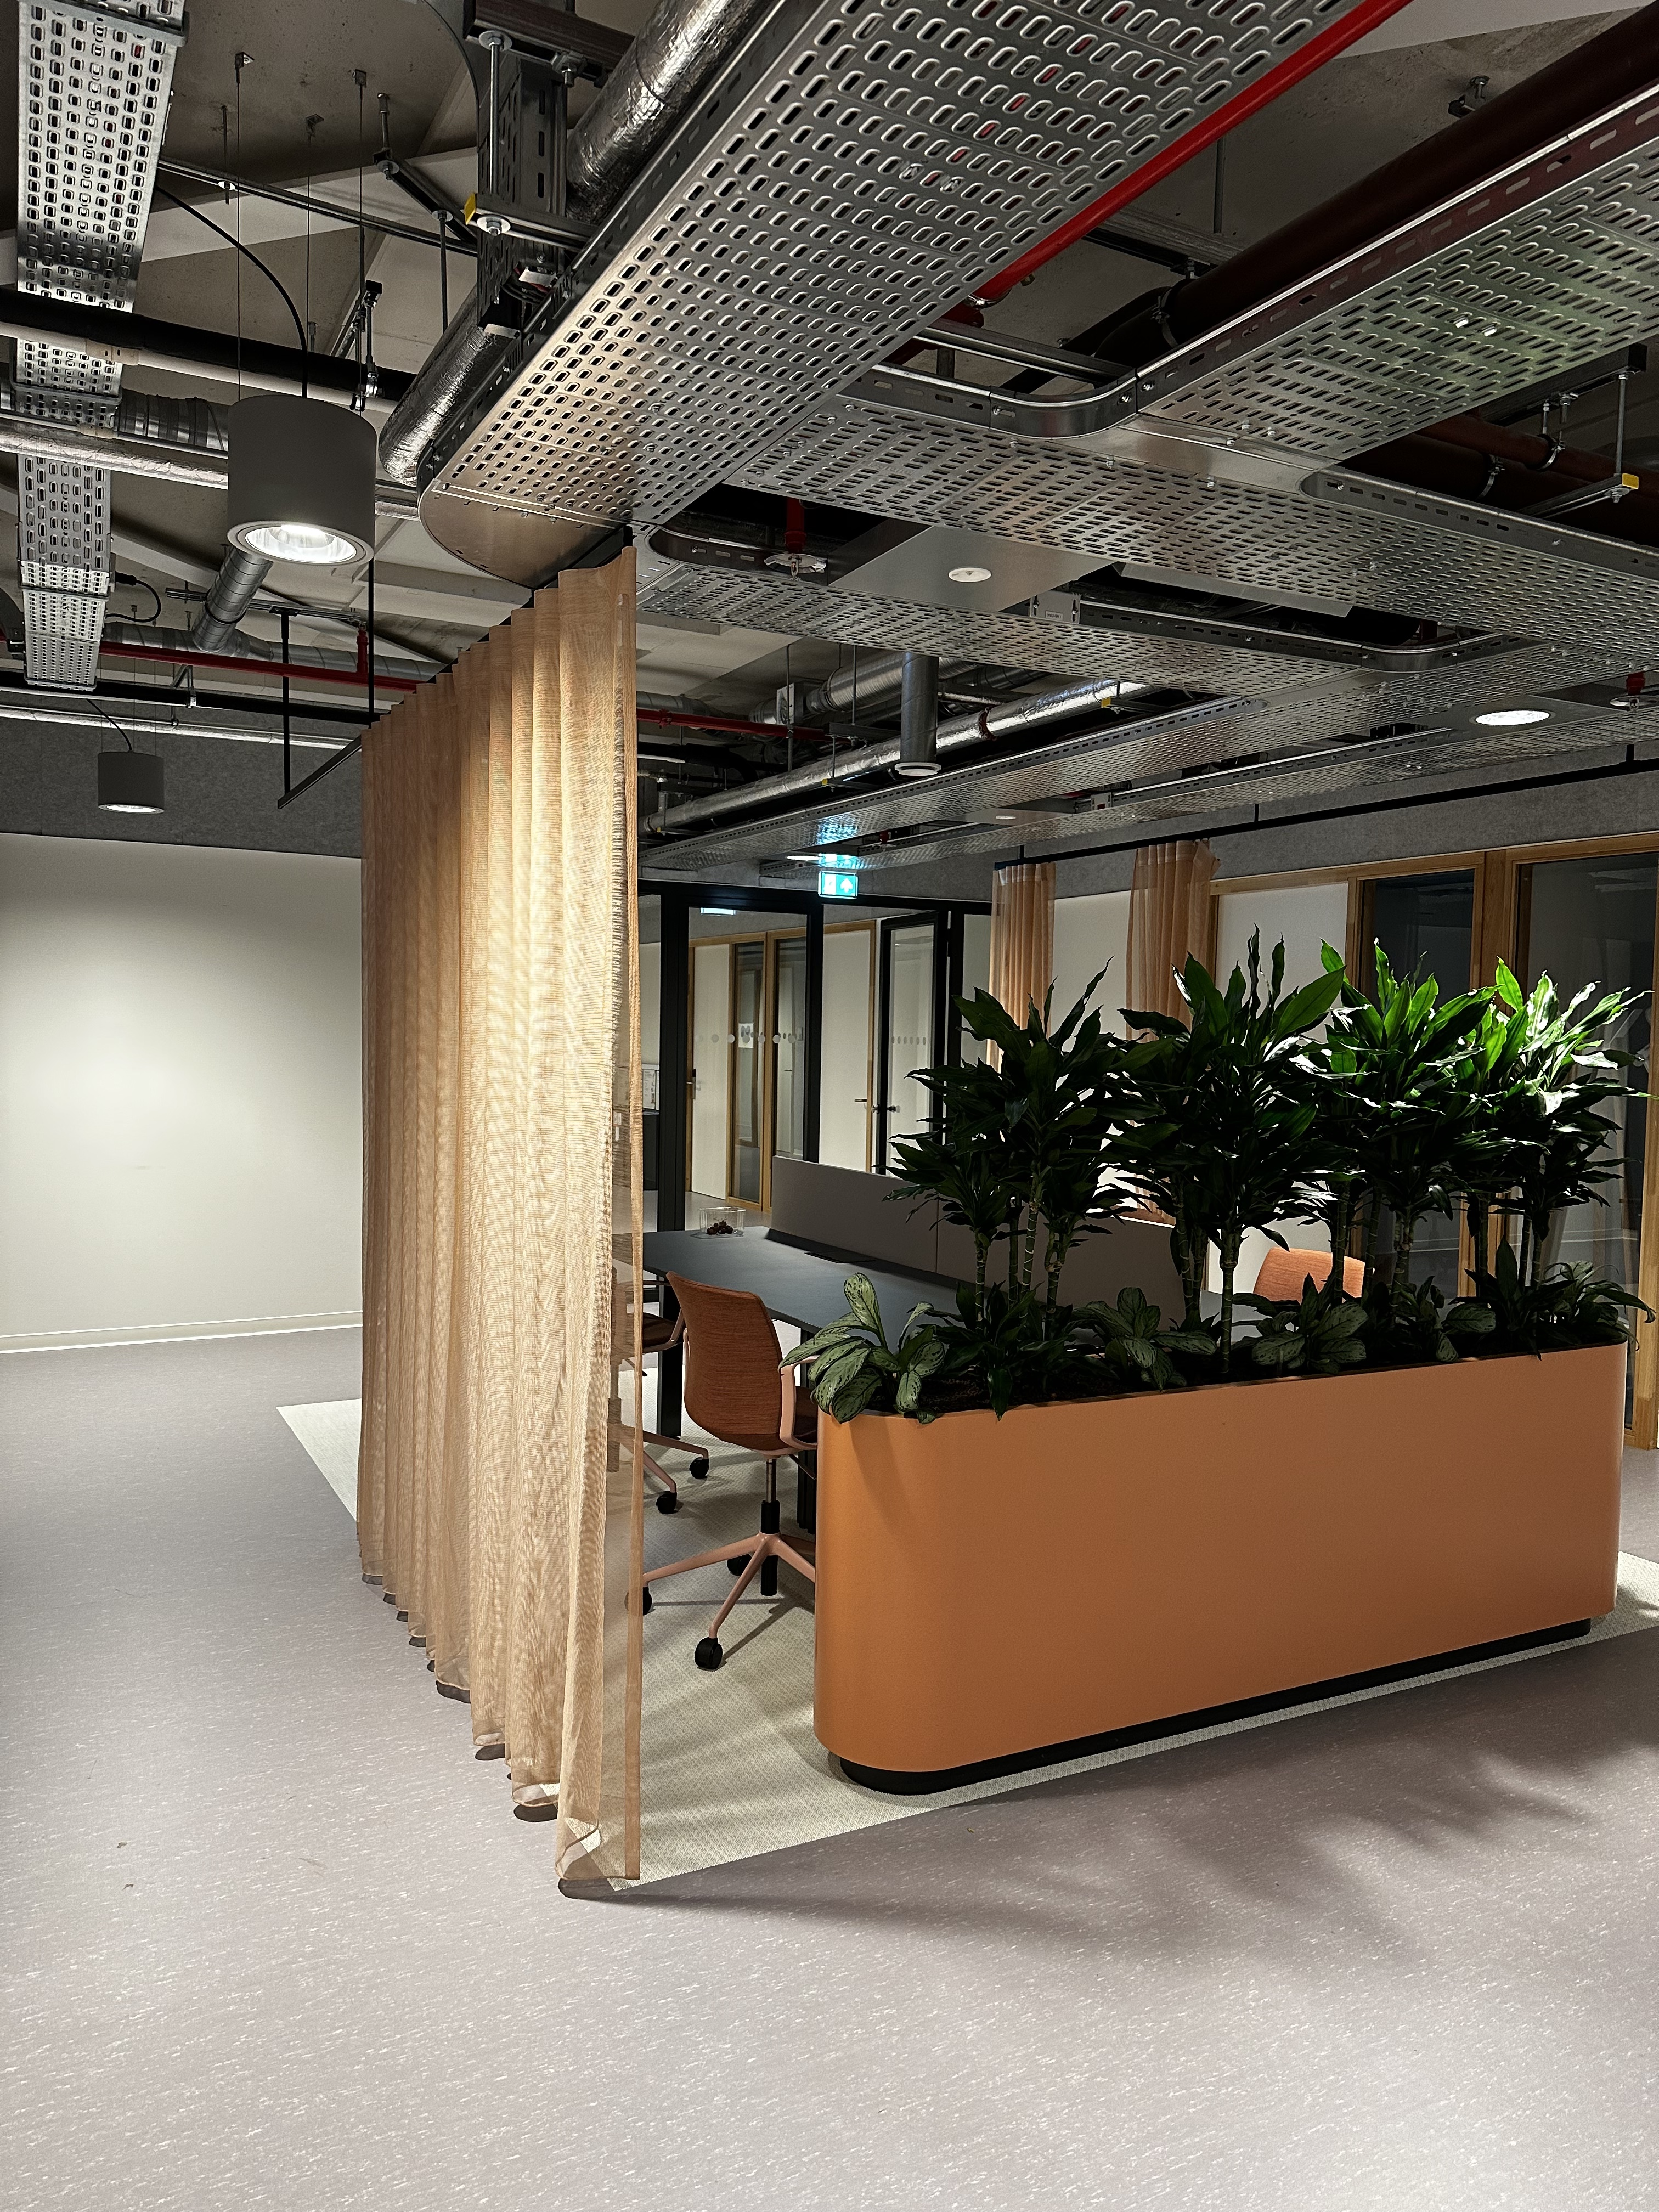
\includegraphics[width=0.5\linewidth]{privacy-curtains.jpg}
%   \end{subfigure}
%   ~
%   \begin{subfigure}
%   \includegraphics[width=0.5\linewidth]{privacy-curtains-fabric.jpg}
%   \end{subfigure}
  
%   \begin{subfigure}
%   \includegraphics[width=0.5\linewidth]{stairs.jpg}
%   \end{subfigure}
%   ~
%   \begin{subfigure}
%   \includegraphics[width=0.5\linewidth]{stairs-closeup.jpg}
%   \end{subfigure}
%   \caption{1907 Franklin Model D roadster. Photograph by Harris \& Ewing, Inc. [Public domain], via Wikimedia Commons.}
%   \Description{A woman and a girl in white dresses sit in an open car.}
% \end{figure}


Our motivation to understand the ``human-building-material" interaction comes from occupying and experiencing one such digital building that houses students, researchers, entrepreneurs, and businesses under one roof. The building labelled as an ``intelligent hub" was designed with a very specific architectural vision to be sustainable, circular and flexible, healthy, and inspiring. To that end, different artifacts in the interior and exterior have been designed using a variety of materials and design features. The building facade itself comprises a pattern of open and closed panels that converge towards the top of the building, referencing a binary code. On the inside, wooden laminated beams contrast floors of recycled concrete. The building aims to encourage meeting and ‘dynamism’ in the lower floors - a glass atrium is used to indicate the feeling of transparency to occupants who can view all ongoing activities of the building. A combination of unusual and lively plinth is designed to make occupants feel curious and stimulate curiosity. Quiet and high-concentration in the upper zones are indicated by recycled PET felt fashioned into panels, and inner walls to promote acoustics. A combination of intelligent sensors throughout the building control light, temperature, and air quality to provide for comfort based on available number of occupants. 


Here we show three tangible artifacts in the building designed to provide experiences using a combination of design and materials, but raise questions about the nature of their role in interacting with the building occupants. We speculate on the analysis of material experiences pattern by applying the four levels of the framework.

\subsubsection*{The Privacy Curtains}
The first artefact is the curtains around high-concentration work spaces. The curtains itself invoke an immediate association with privacy around the workspace (\textit{sensorial level}). However, upon further examination, the sheer material instils a feeling of transparency (\textit{interpretive level}). Therefore, the clash between the concept of privacy and a sheer curtain creates a feeling of confusion and frustration regarding its purpose (\textit{affective level}). However, the physical task of drawing the curtain aids in indicating the need for privacy (\textit{performative level}). So while the curtains itself enable the concept of privacy, the materials themselves create an affective discord. We envision an alternative, smart fabric that can intelligently transform from sheer to fully opaque to in-situ cater to privacy needs.

\subsubsection*{An Encouraging Staircase}
The building promotes their staircase as being designed to inspire people to climb stairs rather than use a lift. However, cold and textured wrought iron railings discourages one from using it (\textit{sensorial level}). The black, oversized, and floating structure floating, casts a foreboding  shadow on the onlooker  (\textit{interpretive level}) and the brutalist design evokes a feeling of awe - something to observe, rather than use (\textit{affective level}). We find that the staircase often fails to create a feeling of encouragement.

\subsubsection*{}
A large screen in the building foyer accompanied by an interactive interface allows users to explore and learn different things about the building. The interface is an interactive tablet that can be accessed by clicking and moving information around (\textit{sensorial level}). The screen presents itself a digital building attempting to serve as a transparent unravel the black-box  nature of intelligent technologies (\textit{interpretive level}). This placement triggers intrigue about learning more about the building (\textit{affective level}). However, limited information displayed prevents the device from becoming part of a daily practice (such as checking ones phone) (\textit{performative level}). 


% Our proposed case study
\subsection{Our Proposed Case Study} 
Towards understanding the impact of digital and non-digital materials on occupants in smart buildings, we are undertaking a preliminary case study in the above discussed building.
We aim to identify occupants' novel and subjective experiences (such as comfort and emotions) that arise from interactions within the smart building. We wish to thereafter identify specific influential factors (tangible and intangible) that determine the overall sense of comfort and emotions in smart buildings spaces. The case study comprises two phases: (a) emotion and comfort label collection, and (b) building walk. First, we will conduct a short survey to obtain a large number of occupant emotion and comfort information regarding different spaces in the building. Next, a building walk will be organised to obtain an in-depth understanding of occupants' perceptions - mental, emotional and physical towards different spaces in the building. During the walk, researchers will engage participants in conversations about each space, and conversations will follow the materials experience framework to understand the relationship between materials, occupants and practises within the differnt spaces of the building \cite{giaccardi2015foundations}. Questions will also investigate the four different experiential levels (sensory, interpretive, affective and per formative) and will include asking about impressions of the space, usage of space \textit{(How would you use this space? Why do you use this space? What kind of tasks would you perform in this space?)}, emotions in the space \textit{(What emotions do you associate with this space?)}, comfort \textit{(Is this space comfortable? Is there sufficient light, warmth, ventilation?)}, shortcomings and scope for improvement. Participants will also be encouraged to take photos of artifacts that stand out to them. Data collected from both phases will be analysed using thematic analysis, and lexical analysis \cite{braun2006using, xue2020mood}. 


% Expected outcomes that can inform B X M research - Material as a catalyst for human action
\subsection{Expected Contributions}
Through our case study, we aim to (among other goals) identify specific artifacts both tangible and intangible, and the material properties of these artifacts that impact building occupants. Additionally, we expect to gain an understanding of the lived-in bodily comfort and emotional experiences within smart buildings. We believe that our findings may help put forth considerations for designing for occupants needs in smart buildings through the lens of material experiences framework. Our findings may be used for the design and development of materials that can help create experiences that occupants might find lacking in smart buildings (for eg., sense of autonomy and control in an automated building) \cite{moreno2014user}, or enhance certain other experiences (for eg., feeling of groundedness and familiarity in a space used by many) \cite{rehman2022personalisedcomfort}.  For example, smart spaces could be designed with materials that in-situ infer occupants (negative) affective states, and attempt to alter it through means of emapthic responses. 

We ultimately envision a design philosophy for smart, hybrid learning spaces that allow materials to shape technology and the ``smartness" of the space. We wish to use our discussion to bring together research communities of material and interaction design with comfort studies and smart buildings.


\section{Conclusion}
The increased complexity of built environments in recent years can be attributed to a growing expectation for buildings to adapt to changing socio-environmental parameters. Given the inevitable growth of smart buildings, in this position paper we suggest that materials of a space can play a central role in understanding and shaping occupants needs towards more human-centric smart buildings. We discuss how materials (both tangible and intangible) of smart buildings can be examined and designed for occupants subjective needs. To that end, we highlight a case study that we will undertake to identify understand the impact of one such smart building and it's artifacts (tangible and intangible) that impact building occupants, and therefore needs rethinking and  redesign such that they may serve as catalysts for human comfort and mental health. 

\bibliographystyle{ACM-Reference-Format}
\bibliography{affective-comfort}

%%
%% If your work has an appendix, this is the place to put it.

\end{document}
\endinput
%%
%% End of file `sample-authordraft.tex'.


% \section{Figures}

% The ``\verb|figure|'' environment should be used for figures. One or
% more images can be placed within a figure. If your figure contains
% third-party material, you must clearly identify it as such, as shown
% in the example below.
% \begin{figure}[h]
%   \centering
%   \includegraphics[width=\linewidth]{sample-franklin}
%   \caption{1907 Franklin Model D roadster. Photograph by Harris \&
%     Ewing, Inc. [Public domain], via Wikimedia
%     Commons. (\url{https://goo.gl/VLCRBB}).}
%   \Description{A woman and a girl in white dresses sit in an open car.}
% \end{figure}

% \subsection{The ``Teaser Figure''}

% A ``teaser figure'' is an image, or set of images in one figure, that
% are placed after all author and affiliation information, and before
% the body of the article, spanning the page. If you wish to have such a
% figure in your article, place the command immediately before the
% \verb|\maketitle| command:
% \begin{verbatim}
%   \begin{teaserfigure}
%     \includegraphics[width=\textwidth]{sampleteaser}
%     \caption{figure caption}
%     \Description{figure description}
%   \end{teaserfigure}
% \end{verbatim}
